\documentclass[a4paper,10pt]{article}
\usepackage{fullpage}
\usepackage{graphicx}
\usepackage{times}
\usepackage{url}

\begin{document}

\title{L41: Lab 5 - TCP Latency and Bandwidth}
\author{Dr Robert N.M. Watson \and Dr Graeme Jenkinson}
\date{Lent Term 2017}
\maketitle

\noindent
The goals of this lab are to:

\begin{itemize}
\item Learn to draw TCP time-bandwidth and time--sequence-number diagrams
\item Evaluate the effects of latency on effective TCP bandwidth
\item Evaluate the effects of socket-buffer size on effective TCP bandwidth
\end{itemize}

\noindent
Lab 5 builds on investigation started in Lab 4, and uses the same TCP
benchmark.

\section*{Background: TCP, latency, and bandwidth}

The Transmission Control Protocol (TCP) layers an reliable, ordered,
byte-stream service over the Internet Protocol (IP).
As explored in the previous lab, TCP goes through complex setup and shutdown
procedures, but (ideally) spends the majority of its time in the
\texttt{ESTABLISHED} state, in which stream data can be transmitted to the
remote endpoint.
TCP specifies two rate-control mechanisms:

\begin{description}
\item[Flow control] allows a receiver to limit the amount of unacknowledged
  data transmitted by the remote sender, preventing receiver buffers from
  being overflowed.
  This is implemented via \textit{window advertisements} sent via
  acknowledgments back to the sender.
  When using the sockets API, the advertised window size is based on available
  space in the \textit{receive socket buffer}, meaning that it will be
  sensitive to both the size configured by the application (using socket
  options) and the rate at which the application reads data from the buffer.

  Contemporary TCP implementations \textit{auto-resize} socket buffers if a
  specific size has not been requested by the application, avoiding use of a
  constant default size that may substantially limit overall performance (as
  the sender may not be able to fully fill the \textit{bandwidth-delay
  product} of the network).
  Note that this requirement for large buffer sizes is in tension with local
  performance behaviour explored in prior IPC labs.

\item[Congestion control] allows the sender to avoid overfilling the network
  path to the receiving host, avoiding unnecessary packet loss and negative
  impacting on other traffic on the network (\textit{fairness}).
  This is implemented via a variety of congestion-detection techniques,
  depending on the specific algorithm and implementation -- but most
  frequently, interpretation of packet-loss events as a congestion indicator.
  When a receiver notices a gap in the received sequence-number series, it
  will return a \textit{duplicate ACK}, which hints to the sender that a
  packet has been lost and should be retransmitted\footnote{This is one reason
  why it is important that underlying network substrates retain packet
  ordering for TCP flows: misordering may be interpreted as packet loss,
  triggering unnecessary retransmission.}.

  TCP congestion control maintains a \textit{congestion window} on the sender
  -- similar in effect to the flow-control window, in that it limits the
  amount of unacknowledged data a sender can place into the network.
  When a connection first opens, and also following a timeout after
  significant loss, the sender will enter \textit{slow start}, in which the
  window is `opened' gradually as available bandwidth is probed.
  The name `slow start' is initially confusing as it is actually an
  exponential ramp-up.
  However, it is in fact slow compared to the original TCP algorithm, which
  had no notion of congestion and overfilled the network immediately!

  When congestion is detected (i.e., because the congestion window has gotten
  above available bandwidth triggering a loss), a cycle of congestion recovery
  and avoidance is entered.
  The congestion window will be reduced, and then the window will be more
  slowly reopened, causing the congestion window to continually (gently) probe
  for additional available bandwidth, (gently) falling back when it re-exceeds
  the limit.
  In the event a true timeout is experienced -- i.e., significant packet loss
  -- then the congestion window will be cut substantially and slow start will
  be re-entered.

  The steady state of TCP is therefore responsive to the continual arrival and
  departure of other flows, as well as changes in routes or path bandwidth, as
  it detects newly available bandwidth, and reduces use as congestion is
  experienced due to over utilisation.
\end{description}

TCP composes these two windows by taking the minimum: it will neither send too
much data for the remote host, nor for the network itself.
One limit is directly visible in the packets themselves (the advertised
window from the receiver), but the other must either be intuited from wire
traffic, or more preferably, monitored using end-host instrumentation.
Two further informal definitions will be useful:

\begin{description}
\item[Latency] is the time it takes a packet to get from one endpoint to
  another.
  TCP implementations measure \textit{Round-Trip Time (RTT)} in order to tune
  timeouts detecting packet loss.
  More subtlely, RTT also limits the rate at which TCP will grow the
  congestion window, especially during slow start: the window can grow only as
  data is acknowledged, which requires round-trip times as ACKs are received.

\item[Bandwidth] is the throughput capacity of a link (or network path) to
  carry data, typically measured in bits or bytes per second.
  TCP attempts to discover the available bandwidth by iteratively expanding
  the congestion-control window until congestion is experienced, and then
  backing off.
  While bandwidth and latency are notionally independent of one another, they
  are entangled in TCP as the protocol relies on acknowledgments to control
  the rate at which the congestion window is expanded, which is dependent upon
  round-trip time.
\end{description}

\section*{Background: Plotting TCP connections}

For this lab, you will prepare two types of TCP graphs:

\begin{description}
\item[TCP time-bandwidth graphs] plot time on a linear X axis, and bandwidth
  achieved by TCP on a linear or log Y axis.
  Bandwidth may be usefully calculated as the change in sequence number (i.e.,
  bytes) over a window of time -- e.g., a second.
  Care should be taken to handle wrapping in the 32-bit sequence space; for
  shorter measurements this might be accomplished by dropping traces from
  experimental runs in which sequence numbers wrap.

\begin{figure}[t]
\begin{center}
  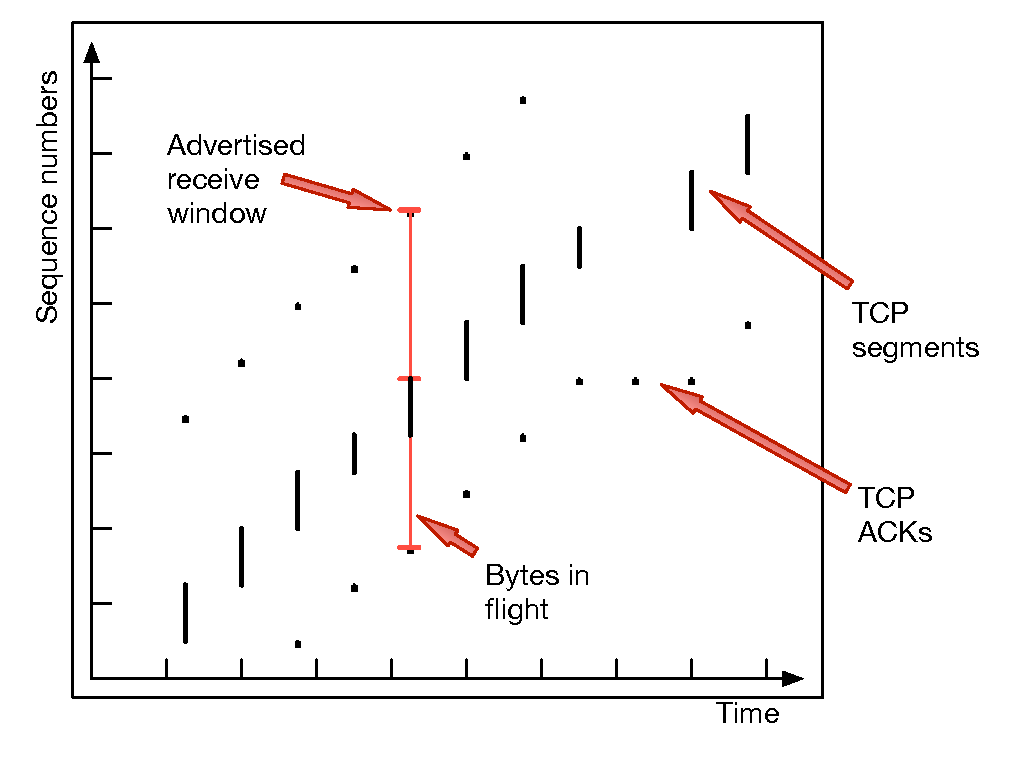
\includegraphics[width=0.75\textwidth]{tcp-time-sequence.pdf}
\end{center}
\caption{TCP time--sequence-number plot: linear X axis representing real time,
and linear Y axis representing the TCP sequence-number space.
TCP segment data is based on the sequence number and segment length from the
sender, and acknowledgement and advertised window based is from the receiver.}
\label{fig:tcp-time-sequence-number-graph}
\end{figure}

\item[TCP time--sequence-number graphs] are a useful means of exploring
  protocol-level behaviour, making a number of important network and protocol
  properties easy to understand visually.
  Figure~\ref{fig:tcp-time-sequence-number-graph} illustrates a somewhat
  abstracted graph with real time on a linear X axis, and the TCP sequence
  space on a linear Y axis -- your graphs will be more concrete (e.g., include
  actual sequence numbers and times!).
  The graph displays properties of a single communication direction in TCP
  (e.g., from server to client), but incorporates data from both data segments
  and their acknowledgments.
  Sender-originated data consists of the range of bytes in a particular TCP
  segment, starting with the transmitted sequence number and continuing
  through the sequence number plus packet length.
  Receiver-originated data consists of the acknowledged sequence number and
  the advertised window (which is added to the acknowledged sequence number
  to calculate the highest sequence number the sender is, at that point,
  allowed to transmit).
\end{description}

Both graphs may benefit from overlaying of additional time-based data, such as
specific annotation of trace events from the congestion-control
implementation, such as packet-loss detection or a transition out of slow
start.
Rather than directly overlaying, which can be visually confusing, a better
option may be to ``stack'' the graphs: place them on the same X axis (time),
horizontally aligned but vertically stacked.
Possible additional data points (and Y axes) miht include advertised and
congestion-window sizes in bytes.
Bandwidth graphs are suitable for plotting quite long periods of protocol
operation, but time--sequence-number graphs will primarily be used when
investigating specific local behaviour in TCP (e.g., around the transition
from slow start to steady state).

\section*{The benchmark}

This lab uses the same IPC benchmark as prior labs.
You will run the benchmark both with, and without, setting the socket-buffer
size, allowing you to explore the effects of manual versus automatic
socket-buffer tuning.
The benchmark continues to send its data on the accepted server-side socket on
port \texttt{10141}.
This means that data segments carrying benchmark data from the sender to the
receiver will have a \textit{source port} of \texttt{10141}, and
acknowledgements from the receiver to the sender will have a
\textit{destination port} of \texttt{10141}.
Do ensure that, as in Lab 2, you have increased the kernel's maximum 
socket-buffer size.

\section*{DTrace probes}

%
% XXXRW: We can't use the normal DTrace TCP send probe because of the limit on
% ARMv7 arguments, so how should students see segments as they are sent --
% without recourse to doing it on the receiver side?  They could use
% ip_output(), but if so will need to check it is a TCP segment first -- and
% on the right port, which is a bit annoying.  We really want the
% higher-numbered arguments.
%
As in Lab 4, you will utilise the \texttt{tcp\_do\_segment} FBT probe to track
TCP input.
However, you will now take advantage of access to the TCP control block
(\texttt{tcpcb} structure -- \texttt{args[3]} to the \texttt{tcp\_do\_segment}
FBT probe) to gain additional insight into TCP behaviour.
The following fields may be of interest:

\begin{description}
\item[\texttt{snd\_wnd}] On the sender, the last received advertised
  flow-control window.
\item[\texttt{snd\_cwnd}] On the sender, the current calculated
  congestion-control window.
\item[\texttt{snd\_ssthresh}] On the sender, the current \textit{slow-start
  threshold} -- if \texttt{snd\_cwnd} is less than or equal to \\
  \texttt{snd\_ssthresh},
  then the connection is in slow start; otherwise, it is in congestion
  avoidance.
\end{description}

When writing DTrace scripts to analyse a flow in a particular direction, you
can use the port fields in the TCP header to narrow analysis to only the
packets of interest.
For example, when instrumenting \texttt{tcp\_do\_segment} to analyse received
acknowledgments, it will be desirable to use a predicate of
\texttt{/args[1]->th\_dport == htons(10141)/} to select only packets being
sent to the server port (e.g., ACKs), and the similar (but subtly different)
\texttt{/args[1]->th\_sport == htons(10141)/} to select only packets being
sent from the server port (e.g., data).
Note that you will wish to take care to ensure that you are reading fields
from within the \texttt{tcpcb} at the correct end of the connection -- the
`send' values, such as last received advertised window and congestion window,
are properties of the server, and not client, side of this benchmark, and
hence can only be accessed from instances of \texttt{tcp\_do\_segment} that
are processing server-side packets.
Unfortunately, using DTrace on ARM, the data length to the \texttt{tcp\_do\_segment} function is not easily available.
To calculate the length of a segment in the probe, you can use the following:

\begin{verbatim}
tdatalen = ntohs(((struct ip *)args[0]->m_data)->ip_len) -
  ((((struct ip *)args[0]->m_data)->ip_hl << 2) +
  (args[1]->th_off << 2));
\end{verbatim}

This D snippet takes the length of the IP datagram and subtracts the combined
lengths of the IP and TCP headers including any options at either layer.
This will be useful in plotting time--sequence-number plots as you will
require both the base sequence number (\texttt{args[1]->th\_seq}) and the
length to calculate the range covered by a transmitted segment.

Data for the two types of graphs described above is typically gathered at (or
close to) one endpoint in order to provide timeline consistency -- i.e., the
viewpoint of just the client or the server, not some blend of the two
time lines.
As we will be measuring not just data from packet headers, but also from the
TCP implementation itself, we recommend gathering most data close to the
sender.
As described here, it may seem natural to collect information on data-carrying
segments on the receiver (where they are processed by
\texttt{tcp\_do\_segment}), and to collect information on ACKs on the server
(where they are similarly processes).
However, given a significant latency between client and server, and a desire
to plot points coherently on a unified real-time X axis, capturing both at the
same endpoint will make this easier.

It is similarly worth noting that \texttt{tcp\_do\_segment}'s entry FBT probe
is invoked before the ACK or data segment has been processed -- so access to
the \texttt{tcpcb} will take into account only state prior to the packet that
is now being processed, not that data itself.
For example, if the received packet is an ACK, then printed \texttt{tcpcb}
fields will not take that ACK into account.

\section*{Flushing the TCP host cache}

FreeBSD implements a \textit{host cache} that stores sampled round-trip times,
bandwidth estimates, and other information to be used across different TCP
connections to the same remote host.
Normally, this feature allows improved performance as, for example, by
allowing past estimates of bandwidth to trigger a transition from slow start
to steady state without `overshooting', potentially triggering significant
loss.
However, in the context of this lab, carrying of state between connections
reduces the independence of our experimental runs.
As such, we recommend issuing the following command (as root) between runs of
the IPC benchmark:

\begin{verbatim}
sysctl net.inet.tcp.hostcache.purgenow=1
\end{verbatim}

\noindent
This will flush all entries from the host cache, preventing information that
may affect congestion-control decisions from being carried between runs.

\section*{Exploratory questions}

These questions are intended to help you understand the behaviours of TCP in
the presence of varying latency and buffer sizes, and may provide supporting
evidence for your experimental questions.
However, they are just suggestions -- feel free to approach the problem
differently!
These questions do not need to be addressed in your lab report.

\begin{enumerate}
  \item As you vary latency between 0ms and 40ms in 5ms increments using
    DUMMYNET, how does overall bandwidth change?
  \item If you pass the \texttt{-s} flag to the IPC benchmark, causing a
    socket option to be issued to modify the socket-buffer size, how does
    this affect the advertised receive window?  You will wish to hold the
    buffer size constant -- we recommend a 1,048,576-byte buffer
    (\texttt{-b 1048576}).
  \item Plot a time--sequence-number graph of a TCP connection with a 10ms
    RTT through shortly after the transition from slow start to steady state.
    Shade any horizontal portions of the graph where \texttt{snd\_cwnd} is
    less than or equal to \texttt{snd\_ssthresh} -- i.e., where TCP is in slow
    start.
    How quickly does TCP reach a steady state -- and is this a product of the
    flow-control window or congestion-control window?
\end{enumerate}

\section*{Experimental questions (part 2)}

These questions supplement the experimental questions in the Lab 4 handout.
Configure the benchmark as follows:

\begin{itemize}
\item To use the statically linked version: \texttt{ipc-static}
\item To use TCP: \texttt{-i tcp}
\item To use a 2-thread configuration: \texttt{2thread}
\item To use a fixed 1MB buffer \texttt{-b 1048576}
\item To set (or not set) the socket-buffer size: \texttt{-s}
\item To use only I/O-loop analysis
\item Flush the TCP host cache between all benchmark runs
\end{itemize}

\noindent
Explore the following experimental questions, which consider only the TCP
steady state, and not the three-way handshake or connection close:

\begin{itemize}
  \item Plot DUMMYNET-imposed latency (0ms .. 40ms in 5ms intervals) on the X
    axis and effective bandwidth on the Y axis, considering both the case
    where the socket-buffer size is set versus allowing it to be auto-resized.
    Is the relationship between round-trip latency and bandwidth linear?
    How does socket-buffer auto-resizing help, hurt, or fail to affect
    performance as latency varies?

  \item Plot a time--bandwidth graph comparing the effects of setting the
    socket-buffer size versus allowing it to be auto-resized by the stack.
    Stack additional graphs showing the sender last received advertised window
    and congestion window on the same X axis.
    How does socket-buffer auto-resizing affect overall performance, as
    explained in terms of the effect of window sizes?

  \item Plot a time--sequence-number graph for two new TCP connections through
    a few packets past the end of slow start for each of the runs, one with a
    10ms round-trip time, and another with a 20ms round-trip time.
    How has latency affected the time required to enter the steady state?
    What is the resulting effect on bandwidth for the two connections over the
    same period?
\end{itemize}

\noindent
Ensure that your final lab report answers all of the experimental questions in
both labs 4 and 5.

\end{document}
